\section{Euclidean formalism}\label{ss:Euclidean}
In this section, we rewrite the definition of entanglement entropy by introducing an auxiliary (replica) parameter.
After giving a representation of the reduced density matrix in terms of the path integral, we derive an expression of the entanglement entropy given by the Euclidean partition function on a singular manifold. 
This approach is sometimes easier than the real time approach in performing analytic computations in QFT.


\subsection{Replica trick}
We adopt the definition Eq.\,\eqref{EE_def} of entanglement entropy with Eqs.\,\eqref{RenyiDef} and \eqref{RenyiEE},
\begin{align}\label{EE_Replica}
\begin{aligned}
S_A &= -\lim_{n\to 1}\frac{\log \tr_A( \rho_A^n)}{n-1} \ ,\\
	&= -\lim_{n\to 1}\partial_n \log \tr_A (\rho_A^n) \ ,
\end{aligned}
\end{align}
where we used the fact that the reduced density matrix is normalized $\tr_A (\rho_A) = 1$.
Although the R{\'e}nyi entropy is defined only for an integer $n$, the analytic continuation is assumed in taking the $n\to 1$ limit.
This method is called the replica trick that is often employed for the entanglement entropy calculation in QFT.


\paragraph*{Two spin system with the replica trick $:$}
We revisit the two spin system Eq.\,\eqref{TwoSpinPure} in Sec. \ref{TwoSpin} with the replica trick.
The reduced density for the spin $A$ was given by Eq.\,\eqref{TwoSpinRD}, hence we immediately have the trace of the $n^{th}$ power,
\begin{align}
	\tr_A (\rho_A^n)  = 2^{1-n} \ .
\end{align}
Plugging this into Eq.\,\eqref{EE_Replica} yields the entanglement entropy
\begin{align}
	S_A = - \lim_{n\to 1} \partial_n \log 2^{1-n} = \log 2 \ ,
\end{align}
which agrees with the previous calculation Eq.\,\eqref{EE_TwoSpin}.




\subsection{Path integral representation in quantum mechanics}
We have seen how the reduced density matrix for entanglement entropy is calculated in the Hamiltonian formulation so far.
There is an equivalent, but complementary approach using the path integral formulation of quantum mechanics which we are going to deal with and will be further extended to quantum field theory in the next section.

We first recap the basic facts about quantum mechanics and the path integral formulation.
In the Schr\"odinger picture a state evolves under the Schr\"odinger equation,
\begin{align}
	\i\, \frac{\d}{\d t}\, |\psi (t)\rangle = \hat H\,  |\psi (t)\rangle \ ,
\end{align}
while operators such as a position operator $\hat x$ do not.
Hence the eigenvector $\hat x |x\rangle = x| x\rangle$ for the operator is also time independent.

In the Heisenberg picture, operators evolve under the Heisenberg equation
\begin{align}
	\i\, \frac{\d}{\d t}\, \hat A(t) = [\hat H, \hat A(t)] \ ,
\end{align}
but the state vectors are time independent.
The operator $\hat x(t)$ and the eigenvector $|x; t \rangle$ are related to those in the Schr{\"o}dinger picture as
\begin{align}
	\hat x(t) &= e^{\i \hat H t}\, \hat x\,e^{-\i \hat H t} \ , \qquad
	|x; t \rangle = e^{\i \hat H t} |x\rangle \ .
\end{align}
The transition amplitude from an initial state $|x_i; t_i\rangle$ at time $t=t_i$ to a final state $|x_f; t_f\rangle$ at $t=t_f (>t_i)$ is given by their overlap $\langle x_f; t_f |x_i; t_i\rangle$ in the Heisenberg picture.
Thus the transition amplitude in the Schr\"odinger picture is
\begin{align}
	\langle x_f; t_f |x_i; t_i\rangle = \langle x_f |\, e^{-\i \hat H(t_f - t_i)}\,|x_i\rangle \ .
\end{align}
A standard argument for splitting the time interval to a number of small intervals and inserting the complete bases at each time slice yields the path integral representation,
\begin{align}\label{QMkernel}
	\langle x_f | e^{-\i \hat H(t_f - t_i)}|x_i\rangle = \int_{x(t_i) = x_i}^{x(t_f) = x_f} [\CD x(t)]\, e^{\i \int_{t_i}^{t_f}\, \d t \,L(x, \dot x)} \ ,
\end{align}
where $L(x, \dot x)$ is the Lagrangian for the system of the given Hamiltonian and $[\CD x(t)]$ is the path integral measure.

We represent the ground state wave function in the path integral language.
It is most easily achieved by analytically continuing the Lorentzian time $t$ to the Euclidean time $\tau$ by the Wick rotation $t = - \i\,\tau$.
The transition amplitude becomes
\begin{align}\label{QMkernelE}
\begin{aligned}
	\langle x_f; \tau_f |x_i; \tau_i\rangle &= \langle x_f | \,e^{-\hat H(\tau_f - \tau_i)}\,|x_i\rangle \ ,\\
		&= \int_{x(\tau_i) = x_i}^{x(\tau_f) = x_f} [\CD x(\tau)]\, e^{- I_E(x)} \ ,
\end{aligned}
\end{align}
where $I_E(x)$ is the Euclidean action.
We specialize the propagator Eq.\,\eqref{QMkernelE} to the case with $(x_f, \tau_f) = (x,0)$ and $(x_i, \tau_i) = (y,T)$, and insert a complete set of the energy eigenstates $\hat H |n\rangle = E_n |n\rangle$ of the Hamiltonian in the left-hand side to obtain
\begin{align}\label{EuclideanAmp}
\begin{aligned}
	\langle x; 0 | y; T\rangle &= \langle x | \,e^{\hat H T}\,|y\rangle \ , \\
			&= \sum_{n} \psi_n (x) \,\psi_n^\ast (y)\, e^{E_n T} \ ,
\end{aligned}
\end{align}
where $\psi_n(x) \equiv \langle x | n\rangle$ is the wave function of the $n^\text{th}$ eigenstate with energy $E_n$.
The transition amplitude Eq.\,\eqref{EuclideanAmp} is dominated by the ground state wave function in $T \to -\infty$ limit,
\begin{align}
	\langle x; 0 | y; -\infty \rangle = \lim_{T\to -\infty} \psi_0(x)\, \psi_0^\ast (y)\, e^{E_0 T} \ .
\end{align}
Multiplying $\psi_0(y)$ and integrating over $y$ using $\int \d y\, |\psi_0(y)|^2 = 1$, 
we obtain the path integral representation of the ground state wave function $\psi_0 (x)$ at $\tau =0$
\begin{align}
	\psi_0 (x) =  \int dy \int_{x(-\infty) = y}^{x(0) = x} [\CD x(\tau)]\, e^{- I_E(x)}\,\psi_0(y) \ , 
\end{align}
where we set $E_0 = 0$ for simplicity.
We make a change of the notation and use $\Psi(x) \equiv \psi_0(x)$ for the ground state wave function from now on.
Also we write the path integral without specifying the boundary condition at $\tau = -\infty$,
\begin{align}\label{GSWFQM}
	\Psi (x) = \int_{\tau=-\infty}^{\tau = 0,\, x(0) = x} [\CD x(\tau)]\, e^{- I_E(x)} \ .
\end{align}
Similarly, the complex conjugate of the ground state wave function is given by the path integral from $\tau = 0$ with a given boundary condition to $\tau = \infty$,
\begin{align}\label{GSWFQMC}
	\Psi^\ast (x) = \int^{\tau=\infty}_{\tau = 0,\, x(0) = x} [\CD x(\tau)]\, e^{- I_E(x)} \ .
\end{align}

We are now in position to apply the path integral representation to calculating the entanglement entropy.
Suppose the system is at zero temperature and in a pure (not necessarily normalized) ground state $|\Psi\rangle$.
The Hilbert space is described by the density matrix $\rho_\text{tot} = |\Psi\rangle\langle \Psi | / Z$ with the partition function $Z\equiv \langle \Psi | \Psi\rangle$ and the reduced density matrix $\rho_A$ becomes
\begin{align}\label{RedDM}
\rho_A = \frac{1}{Z}\,\tr_B (|\Psi\rangle \langle \Psi |) \ .
\end{align}
We consider a bipartite system of two particles whose coordinates are denoted by $x_A$ and $x_B$.
Then a state in the total system is spanned by a tensor product state $|x_A, x_B\rangle \equiv |x_A\rangle\otimes |x_B\rangle$, with which
the matrix element of the reduced density matrix $\rho_A$ is written as
\begin{align}\label{DM_pathinte}
\begin{aligned}
	\langle x_A| \,\rho_A\, |x_A' \rangle &= \frac{1}{Z} \int \d x_B\, \langle x_A, x_B |\Psi\rangle \langle \Psi |x_A', x_B\rangle \ ,
\end{aligned}
\end{align}
where the partial trace over the Hilbert space $B$ is taken by the integration over $x_B$.
We substitute into Eq.\,\eqref{DM_pathinte} the path integral representations Eqs.\,\eqref{GSWFQM} and \eqref{GSWFQMC} of the ground state, but slightly shift the Euclidean time from $\tau = 0$ to $\tau = -\epsilon$ for $\Psi(x)$ and $\tau = \epsilon$ for $\Psi^\ast(x)$ with a small parameter $\epsilon>0$ as a regularization,
\begin{align}
\begin{aligned}
	\langle x_A| &\,\rho_A\, |x_A' \rangle 
		= \frac{1}{Z} \int \d x_B\\ 
		& \cdot \int_{\tau=\epsilon, \text{bc}^+}^{\tau=\infty}\int^{\tau=-\epsilon, \text{bc}^-}_{\tau=-\infty} [\CD y_A(\tau)\,\CD y_B(\tau)]\, e^{- I_E (y_A, y_B)} \ ,
\end{aligned}
\end{align}
where $\text{bc}^\pm$ are the boundary conditions at $\tau = \pm \epsilon$ specified by
\begin{align}
\begin{aligned}
	\text{bc}^+ &=\{ y_A(\epsilon) = x_A', y_B(\epsilon) = x_B\} \ , \\
	\text{bc}^- &= \{y_A(-\epsilon) = x_A, y_B(-\epsilon) = x_B \}\ .
\end{aligned}
\end{align}
Performing the $x_B$ integral and letting $\epsilon$ be zero amounts to the path integral for $y_B$ over the entire Euclidean time while the boundary conditions for $y_A$ at $\tau = \pm \epsilon$ can be implemented by inserting delta functions
\begin{align}\label{QM_rhoA}
\begin{aligned}
	\langle x_A| \,\rho_A\, |x_A' \rangle = \frac{1}{Z} \int^{\tau=\infty}_{\tau=-\infty} &[\CD y_A(\tau)\,\CD y_B(\tau)]\,e^{- I_E (y_A, y_B)}\\
	&\cdot \delta \left[ y_A(0^+) - x_A'\right]\,\delta \left[ y_A(0^-) - x_A\right]\ , 
\end{aligned}
\end{align}
where we introduced the notation $0^\pm =\lim_{\epsilon\to +0}\pm\epsilon$.
Eq.\,\eqref{QM_rhoA} leads to the path integral representation of the entanglement entropy, but we postpone the derivation until the next section where we focus on the QFT case.



\subsection{Path integral representation of entanglement entropy in quantum field theory}
The real time formalism is not effective for QFT unless we discretize the space to lattices, and the reduced density matrix is not so straightforward to obtain in QFT.
We want to make use of the path integral representation and represent the entanglement entropy in terms of the partition function on a manifold with a singularity on the entangling surface.

\begin{table}[htbp]
\caption{\label{tab:QM_QFT}Correspondence between quantum mechanics (QM) and quantum field theory (QFT).}
\begin{ruledtabular}
\begin{tabular}{ccc}
  & QM & QFT\\ \hline
 Variable & $\hat x$ & $\hat \phi(\vec x)$\\
 State & $|x\rangle$ & $|\phi (\vec x)\rangle$ \\
 Wave function & $\Psi(x)$ & $\Psi[ \phi(\vec x) ]$
\end{tabular}
\end{ruledtabular}
\end{table}

To this end, we need a representation of the ground state wave function in the path integral form as in the quantum mechanical case.
In QFT$_d$, the variable corresponding to the coordinate $\hat x$ in QM is a quantum field $\hat\phi(\vec x)$ living on a $(d-1)$-dimensional space parametrized by the coordinate vector $\vec x$ and the state vector obeying the Schr{\"o}dinger equation is the eigenvector of the field operator $\hat \phi (t,\vec{x})$ at $t=0$: $\hat \phi (0,\vec{x}) |\phi_0(\vec{x}) \rangle = \phi_0(\vec{x})|\phi_0(\vec{x}) \rangle$ (see Table \ref{tab:QM_QFT}).


In QFT the wave function of the ground state $|\Psi\rangle$ is given by the wave functional $\Psi \left[\phi_0(\vec{x})\right] = \langle \phi_0(\vec{x}) |\Psi\rangle$ whose Euclidean path integral representation is
\begin{align}
\begin{aligned}
\Psi \left[\phi_0(\vec{x})\right] &= \langle \phi_0(\vec{x}) |\Psi\rangle \ ,\\
	&= \int_{t=-\infty}^{t=0, \, \phi(t=0,\vec{x}) = \phi_0 (\vec{x})} [\CD\phi (t,\vec{x})] \,e^{-I_E[\phi]} \ .
\end{aligned}
\end{align}
Similarly, we can represent the conjugate of the wave functional by
\begin{align}
\begin{aligned}
\Psi^\ast \left[\phi_0'(\vec{x})\right] &=\langle\Psi |\phi_0'(\vec{x})\rangle \ ,\\
	&= \int_{t=0,\,\phi(t=0,\vec{x}) = \phi_0' (\vec{x})}^{t=\infty} [\CD\phi (t,\vec{x})] \,e^{-I_E[\phi]} \ .
\end{aligned}
\end{align}
Figure \ref{fig:wavefunc} shows the pictorial representations of the wave functionals.
%
\begin{figure}[h]
\centering
	\begin{tikzpicture}[scale = 0.8]
			\draw[fill=verylightgray, thick] (-3, 0) -- node[below] {$t=0$} node[above]{$\phi_0$} (-1, 0) -- (-1, -2) -- node[below]{$t=-\infty$} (-3, -2) -- (-3, 0);
			\draw[dashed, thick] (-3, 0) -- (-3, 2) -- node[above] {$t=\infty$} (-1, 2) -- (-1, 0);
			\node at (-4, 0) {$\langle \phi_0 |\Psi\rangle =$};
			\draw[->, thick] (-3.1, -3) -- (-0.9, -3) node[right] {$\vec{x}$};
			\draw[->, thick] (-0.5, -2) -- (-0.5, 2.1) node[above] {$t$};			
	\end{tikzpicture}
	\hspace*{0.5cm}
	\begin{tikzpicture}[scale = 0.8, xshift=-0.5cm]
			\draw[fill=verylightgray, thick] (3, 0) -- node[above] {$t=0$} node[below]{$\phi_0'$} (5, 0) -- (5, 2) -- node[above]{$t=\infty$} (3, 2) -- (3, 0);
			\draw[dashed, thick] (3, 0) -- (3, -2) -- node[below] {$t=-\infty$} (5, -2) -- (5, 0);
			\node at (2, 0) {$\langle \Psi | \phi_0' \rangle =$};
			\draw[->, thick] (2.9, -3) -- (5.1, -3) node[right] {$\vec{x}$};
			\draw[->, thick] (5.5, -2) -- (5.5, 2.1) node[above] {$t$};	
	\end{tikzpicture}
\caption{\label{fig:wavefunc} Path integral representations of a wave function.
The integral is performed over the shaded regions.}
\end{figure}
%
The partition function $Z$ is the path integral over the entire Euclidean space as it is written by
\begin{align}
	Z = \int [\CD \phi_0(t=0, \vec x)]\, \langle \Psi | \phi_0 \rangle \,\langle\phi_0| \Psi\rangle \ .
\end{align}
In this pictorial expression, taking the partial trace over the subsystem $B=\bar A$ is equivalent to gluing the edges of the two sheets $\langle\Psi|\phi_0\rangle$ and $\langle \phi_0 |\Psi\rangle$ along $B$.
%
In other words, this is implemented by integrating the total density matrix over every state $\phi^B(t=0,\vec{x})$ with support only on $\vec{x}\in B$: 
\begin{align}
\rho_A = \frac{1}{Z} \int [\CD \phi^B(t=0, \vec{x}\in B)] \langle \phi^B| \Psi \rangle \langle \Psi | \phi^B\rangle \ .
\end{align}
The reduced density matrix has two indices $[\rho_A]_{ab} = \langle \phi_a^A |\rho_A |\phi_b^A\rangle$ where $\phi_a^A(\vec{x}\in A)$ and $\phi_b^A(\vec{x}\in A)$ specify the boundary conditions on $A$ at $t=0^+$ and $0^-$, respectively.\footnote{Here the order of the indices of $\rho_A$ is chosen so that the path integral representation looks natural. One may use the opposite order and still obtain the same result.}
Therefore, $\rho_A$ is represented by the path integral on the Euclidean space with a cut along the subsystem $A$,
\begin{align}\label{QFT_RD_PIR}
\begin{aligned}
 &[\rho_A]_{ab} \\
&=
 \frac{1}{Z} \int [\CD \phi^B(t=0, \vec{x}\in B)]\,  \left(\langle \phi_a^A| \langle \phi^B|\right) |\Psi\rangle \langle \Psi |\left( | \phi_b^A \rangle  | \phi^B \rangle \right) \ , \\
&=\frac{1}{Z} \int [\CD \phi^B(t=0, \vec{x}\in B)]\quad  
\begin{tikzpicture}[baseline={([yshift=-.5ex]current bounding box.center)}]
			\draw[fill=verylightgray, thick] (-1, -1.5) -- ++ (3, 0) --++  (0, 1.4) -- node [below] {\textcolor{kakiiro}{$\phi_a^A$}} ++ (-3, 0) --++ (0, -1.4);
			\draw[fill=verylightgray, thick] (-1, 0.1) -- node[above] {\textcolor{hanadairo}{$\phi_b^A$}} ++ (3, 0) --++  (0, 1.4) --++ (-3, 0) --++ (0, -1.4);
			\filldraw [fill=black] (0,0.1) node [above left] {$\phi^B$} circle (0.05);
			\filldraw [fill=black] (1,0.1) node [above right] {$\phi^B$} circle (0.05);			
			\filldraw [fill=black] (0,-0.1) node [below left] {$\phi^B$} circle (0.05);
			\filldraw [fill=black] (1,-0.1) node [below right] {$\phi^B$} circle (0.05);
			\filldraw [fill=black] (0,-1.8) circle (0.05);
			\filldraw [fill=black] (1,-1.8) circle (0.05);
			\node[right] at (2, 0.2) {$t = 0^+$};
			\node[right] at (2, -0.2) {$t = 0^-$};
			\draw[dashed] (0, -0.1) -- (0, -1.8);
			\draw[dashed] (1, -0.1) -- (1, -1.8);
			\draw[thick, ->] (-1, -1.8) -- node[below] {$B\quad~~ A \quad~~B$} (2.1, -1.8) node[right] {$\vec{x}$};
\end{tikzpicture} \\
&=\frac{1}{Z}\quad \begin{tikzpicture}[baseline={([yshift=-.5ex]current bounding box.center)}]
			\draw[fill=verylightgray, thick] (-1, -1.5) -- (2, -1.5) --  (2, 1.5) -- (-1, 1.5) -- (-1, -1.5);
			\draw[thick, ->] (-1, -1.8) -- node[below] {$B\quad~~ A \quad~~B$} (2.1, -1.8) node[right] {$\vec{x}$};
			\filldraw [fill=black] (0,-1.8) circle (0.05);
			\filldraw [fill=black] (1,-1.8) circle (0.05);
			\draw[fill=white, thick] (0, -0.1) -- node[below] {\textcolor{kakiiro}{$\phi_a^A$}} (1, -0.1) -- (1, 0.1) -- node[above] {\textcolor{hanadairo}{$\phi_b^A$}} (0, 0.1) -- (0, -0.1);
			\draw[dashed] (1, -0.1) -- (2, -0.1);
			\draw[dashed] (1, 0.1) -- (2, 0.1);
			\node[right] at (2, 0.2) {$t = 0^+$};
			\node[right] at (2, -0.2) {$t = 0^-$};
			\draw[dashed] (0, -0.1) -- (0, -1.8);
			\draw[dashed] (1, -0.1) -- (1, -1.8);
\end{tikzpicture} \\
&= \frac{1}{Z} \int
[\CD \phi(t,\vec{x})]\, e^{-I_E[\phi]} \\
	&\qquad \cdot  \prod_{\vec{x} \in A} \delta\left( \phi(0^+, \vec{x}) - \phi_b^A(\vec{x})\right)\,\delta\left( \phi(0^-, \vec{x}) - \phi_a^A(\vec{x})\right) \ .
\end{aligned}
\end{align}
While we derived it pictorially here it takes exactly the same form as the quantum mechanical case, Eq.\,\eqref{QM_rhoA}.
In other words, we are able to arrive at the path integral representation Eq.\,\eqref{QFT_RD_PIR} of the reduced density matrix in QFT from the previous result Eq.\,\eqref{QM_rhoA} in QM using the dictionary in Table \ref{tab:QM_QFT}.

It follows from this representation that the trace of $n^{th}$ power of the reduced density matrix 
is given by the partition function $Z_n$ on the $n$-fold cover $\CM_n$ of the original spacetime that is constructed by gluing $n$ copies of the sheet with a cut along $A$ \cite{Holzhey:1994we,Calabrese:2004eu},
\begin{align}\label{Replica_DM_PF}
\begin{aligned}
\tr_A (\rho_A^n) &= \frac{1}{(Z)^n}\qquad 
	\begin{tikzpicture}[baseline={([yshift=-.5ex]current bounding box.center)},scale=0.75, every node/.style={scale=0.85}]
				\draw[fill=verylightgray, thick] (-2, 4) -- (1, 4) -- (2, 5.5) --(-1, 5.5) -- (-2, 4);
				\draw[fill=white] (-0.7, 4.7) -- node[below] {\textcolor{kakiiro}{$\phi_1^A$}}++(1.2, 0) --++ (0.1, 0.15) -- node[above] {\textcolor{hanadairo}{$\phi_2^A$}} ++(-1.2, 0) --++ (-0.1, -0.15);
				\draw[fill=verylightgray, thick] (-2, 2) -- (1, 2) -- (2, 3.5) --(-1, 3.5) -- (-2, 2);
				\draw[fill=white] (-0.7, 2.7) -- node[below] {\textcolor{hanadairo}{$\phi_2^A$}} ++(1.2, 0) --++ (0.1, 0.15) -- node[above] {\textcolor{enjiiro}{$\phi_3^A$}} ++(-1.2, 0) --++ (-0.1, -0.15);
				\draw[dotted, thick] (-0.2, 1.8) -- (-0.2, 0.2);
				\draw[fill=verylightgray, thick] (-2, -1.5) -- (1, -1.5) -- (2, 0) --(-1, 0) -- (-2, -1.5);
				\draw[fill=white] (-0.7, -0.8) -- node[below] {\textcolor{ebicha}{$\phi_n^A$}} ++(1.2, 0) --++ (0.1, 0.15) -- node[above] {\textcolor{kakiiro}{$\phi_1^A$}} ++(-1.2, 0) --++ (-0.1, -0.15);
				\draw [decorate,decoration={brace,amplitude=10pt,raise=4pt},yshift=0pt]
(2, 5.5) -- (2, -1.5) node [black,midway,right=0.5] {$n$ copies $\equiv Z_n$};
			\end{tikzpicture} \\
	&= \frac{Z_n}{(Z)^n} \ ,
\end{aligned}
\end{align}
where we denote the partition function on the $n$-fold cover by $Z_n$.
Substituting this representation to Eq.\,\eqref{EE_Replica} gives an alternative definition of entanglement entropy in QFT,
\begin{align}\label{EE_PF}
S_A = -\lim_{n\to 1} \partial_n (\log Z_n - n \log Z) \ .
\end{align}
The $n$-fold cover $\CM_n$ has a conical singularity along the codimension-two {\it entangling surface} $\Sigma = \partial A$ with a deficit angle $2\pi (1-n)$.
This expression will be used in later sections.


It is interesting and valuable to give the path integral representation of the modular entropy in Eq.\,\eqref{ModularEntropy} to manifest the relation to thermal entropy.
If we regard $\beta = 2\pi n$ as an inverse temperature, the thermal partition function $Z(\beta)$ defined by Eq.\,\eqref{Thermal_PF} is proportional to the partition function on the singular manifold $\CM_n$,
\begin{align}
	Z(\beta) = \frac{Z_n}{(Z)^n} \ .
\end{align}
The modular entropy $\tilde S_n$, when written in terms of the replica partition function, then becomes
\begin{align}
	\tilde S_n 	= (1- n\partial_n) \log Z_n \ ,
\end{align}
which reduces to the entanglement entropy Eq.\,\eqref{EE_PF} in the $n\to 1$ limit.
Finally performing the integral Eq.\,\eqref{Renyi_Modular} gives the R{\'e}nyi entropy
\begin{align}\label{Renyi_QFT}
	S_n = \frac{1}{1-n}\,\log \left(\frac{Z_n}{Z^n}\right) \ ,
\end{align}
which can also be obtained more directly using Eq.\,\eqref{Replica_DM_PF} and the definition of the R{\'e}nyi entropy, Eq.\,\eqref{RenyiDef}.



\subsection{Entanglement entropy across a hyperplane}
The Euclidean version of the action Eq.\,\eqref{Scalar_action_L} for a free massive scalar field is
\begin{align}
I_E = \frac{1}{2}\int \d^d x \left[ (\partial_\mu \phi)^2 + m^2 \phi^2\right] \ .
\end{align}
We denote the space and Euclidean time coordinates by $x_i\, (i=1,\cdots, d-1)$ and $x_0$.
Let $A$ and $B$ be regions in $x_1> 0$ and $x_1\le0$, respectively.
The entangling surface $\Sigma$ is chosen to be a $(d-2)$-dimensional hyperplane at $x_1=0$: $\Sigma = \{ (x_0 ,x_i)|\, x_0 = x_1 = 0\}$.
Introducing the metric in the polar coordinates for the $(x_0 ,x_1)$ plane,
\begin{align}\label{EE_Hyperplane}
\begin{aligned}
\d s^2 &= \d x_0^2 + \d x_1^2  + \sum_{i=2}^{d-1} \d x_i^2 \ ,\\
 	&= \d r^2 + r^2 \d\tau^2 + \sum_{i=2}^{d-1} \d x_i^2 \ ,
\end{aligned}
\end{align}
the $n$-fold cover $\CM_n$ with a cut along $A$ is given by the same metric with $0\le r$ and $0\le \tau \le 2\pi n$ as shown in Fig.\,\ref{fig:ScalarInfinite}.\footnote{The angular variable $\tau$ should not be confused with the Euclidean time. It is rather considered as the ``modular time" for the modular Hamiltonian.}
Hence the manifold $\CM_n$ is the direct product of the two-dimensional cone $\CC_n$ parametrized by $(r,\tau)$ and $\BR^{d-2}$.
\begin{figure}[htbp]
\centering
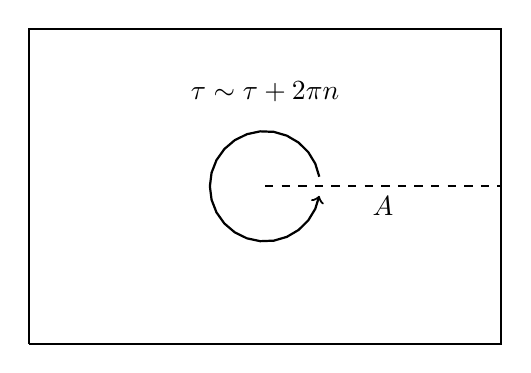
\begin{tikzpicture}
\draw [thick] (0,0) --++ (6,0) --++ (0,4) --++ (-6,0) --++ (0,-4);
\draw [thick, dashed] (3,2) -- node [below] {$A$}++ (3,0); 
\draw [thick, ->, domain=10:350] plot ({3+0.7*cos(\x)}, {2+0.7*sin(\x)});
\node at (3,3.2) {$\tau \sim \tau +2\pi n$};
\end{tikzpicture}
\caption{\label{fig:ScalarInfinite} The $n$-fold cover of $\BR^d$ with a cut along the subregion $A$ ($x_1>0$) at $t=0$ in the polar coordinates.}
\end{figure}

We are concerned with the partition function $Z_n$ of the free scalar field on $\CM_n$, which is simply given by the one-loop determinant
\begin{align}\label{SchwingerRep}
\begin{aligned}
\log Z_n &= -\frac{1}{2} \log \det (-\nabla^2 + m^2) \ , \\
	&= -\frac{1}{2}\tr \log (-\nabla^2 + m^2) \ , \\
	&= \frac{1}{2}\int_{\epsilon^2}^\infty \frac{\d s}{s}\, \tr \left[ e^{-s (-\nabla^2 + m^2)} - e^{-s} \right]\ , 
\end{aligned}
\end{align}
where $\nabla$ is the covariant derivative on $\CM_n$ and we introduced the Schwinger parameter $s$ in the third equality.\footnote{
This follows from the identity for a matrix $M$,
\begin{align}
\log M =  \int_0^\infty \frac{\d s}{s}\left[ e^{-s} - e^{-s M}\right] \ .
\end{align}}
The parameter $s=\epsilon^2\ll 1$ is introduced so as to act as a regulator for the UV divergence.

In the Schwinger representation Eq.\,\eqref{SchwingerRep} the calculation of the partition function amounts to evaluating the kernel in the integrand.
This is straightforward to carry out once the eigenvalues of the Laplacian $\nabla^2$ are given, but finding the eigenfunctions is a formidable task on the $n$-fold cover $\CM_n$ of a general type of entangling surfaces.
Fortunately, the manifold $\CM_n$ for the hyperplanar entangling surface has the direct product structure $\CM_n = \CC_n \times \BR^{d-2}$ as seen from Eq.\,\eqref{EE_Hyperplane}; thus the Laplacian decomposes into the sum of those on $\CC_n$ and $\BR^{d-2}$: $\nabla^2 = \nabla^2_{\CC_n} + \nabla^2_{\BR^{d-2}}$.
We know the plane waves are the eigenfunctions of the flat space Laplacian $\nabla^2_{\BR^{d-2}}$, and we only need to solve the eigenvalue problem for the cone Laplacian $\nabla^2_{\CC_n}$.

The rotational symmetry of the cone $\CC_n$ allows the Fourier decomposition by the modes $\exp (\i\, l \tau/n)$ with integer $l$ along the angle $\tau$ of period $2\pi n$; hence the eigenfunctions $\phi_{k,l}(r,\tau)$ of the Laplacian are parametrized by two parameters $(k, l)$ satisfying
\begin{align}
\begin{aligned}
\nabla^2_{\CC_n} \phi_{k,l}(r,\tau) &= - k^2 \,\phi_{k,l}(r,\tau) \ , \qquad (k\in \BR^+, l\in \BZ) \ , \\
\phi_{k,l}(r,\tau) &= \sqrt{\frac{k}{2\pi n}} \, e^{\i l \tau/n} J_{\left| l/n\right|} (k\,r) \ , 
\end{aligned}
\end{align}
where $J_n$ is the Bessel function of the first kind.
We normalize the eigenfunctions so that they form an orthonormal basis on the cone $\CC_n$ \cite{Kabat:1995eq},
\begin{align}
\int_{\CC_n} \d^2 x\, \phi_{k,l}(x)\, \phi_{k',l'}^\ast (x) &= \delta_{l l'}\, \delta (k - k') \ .
\end{align}
The Laplacian on $\BR^{d-2}$ has the orthonormal basis of the eigenfunctions spanned by the plane waves, $\phi_{{\bm k}^\perp} (y) = \exp (\i\, {\bm k}_\perp \cdot {\bm y}) / (2\pi)^{(d-2)/2}$, with the eigenvalues $-k_\perp^2$.
Thus we can construct the orthonormal basis $\phi_{k,l,{\bm k}_\perp} (x,y) \equiv \phi_{k,l}(x)\, \phi_{{\bm k}_\perp}(y)$ of the Laplacian $\nabla^2$ with the eigenvalues $k^2 + k_\perp^2$, and evaluate the trace of the kernel $\tr\,[e^{-s (-\nabla^2 + m^2)}]$ that appeared in the third line of Eq.\,\eqref{SchwingerRep}:
\begin{align}\label{SLTrace}
\begin{aligned}
\tr &\left[e^{-s (-\nabla^2 + m^2)}\right] \\
	&= \int_{\CC_n} \d^2 x \sum_{l=-\infty}^\infty \int_0^\infty \d k \, e^{-s(k^2 + m^2)} \phi_{k,l}(x)\phi_{k,l}^\ast (x) \\	
		&\qquad \cdot \int_{\BR^{d-2}} \d^{d-2} y \int \d^{d-2}k_\perp \, e^{-s\, k_\perp^2} \, \phi_{{\bm k}^\perp} (y)\phi_{{\bm k}^\perp}^\ast (y) \ ,\\
	&= \frac{\text{Vol}(\BR^{d-2})}{12\, n} \frac{e^{-s m^2}}{(4\pi s)^{(d-2)/2}} \ .
\end{aligned}
\end{align}

There are technical subtleties in performing the integral in Eq.\,\eqref{SLTrace} associated with the UV and IR divergences, each coming from the angular modes $l$ and the volume of the spacetime, respectively. 
One way to see the IR divergence is to use the identity for the calculation that holds for $\text{Re} \,(\alpha) > -1$,
\begin{align}
\int_0^\infty \d k\, k\, e^{-s k^2} J_\alpha (kr)^2 &= \frac{e^{- r^2/(2s)}}{2s}\, I_\alpha \left( \frac{r^2}{2s}\right) \ ,\\
\int_0^\infty \d r\, r \,e^{-r^2} I_\alpha \left( r^2\right) &= - \frac{\alpha}{2} + \int_0^\infty \d r \,\frac{1}{\sqrt{2\pi}} \ ,\label{IR_Identity}
\end{align}
where $I_\alpha$ is the modified Bessel function of the first kind.
The second term on the right-hand side of Eq.\,\eqref{IR_Identity} is divergent, but independent of $\alpha\, (=|l/n|)$, thus giving rise to a term proportional to $n$ from the volume of $\CM_n$ to $\log Z_n$ and does not contribute to the entanglement entropy.
On the other hand, the UV divergence arises from the summation over the angular momentum $l$, which can be regularized, for example, by using the zeta function,
\begin{align}
\sum_{l=-\infty}^\infty |l| = 2\zeta(-1) =  - \frac{1}{6} \ .
\end{align}

Our derivation of Eq.\,\eqref{SLTrace} is slightly different from the one given by \textcite{Kabat:1995eq} that employs another regularization scheme.
An alternative way to evaluate the partition function $Z_n$ is to take a derivative with respect to $m^2$ and find the coincident Green function $G_n(x, x)$ on the $n$-fold cover space $\CM_n$ \cite{Calabrese:2004eu},
\begin{align}
\frac{1}{m^2} \log Z_n = - \frac{1}{2}\int_{\CM_n} \d^dx\, G_n(x, x) \ .
\end{align}


We are left with the other kernel $\tr \,(e^{-s})$ to evaluate in Eq.\,\eqref{SchwingerRep}, but it is easily seen to be proportional to $n$ due to the volume of the cone $\CC_n$ and does not contribute to Eq.\,\eqref{EE_PF} in contrast to Eq.\,\eqref{SLTrace}.
Thus, by putting all together, we obtain the entanglement entropy across a hyperplane $\BR^{d-2}$ for a free massive scalar field,
\begin{align}
	S_A = \frac{\pi\,\text{Vol}(\BR^{d-2})}{3} \int_{\epsilon^2}^\infty \d s \, \frac{e^{-s m^2}}{(4\pi s)^{d/2}}  \ .
\end{align}

The UV divergent terms of the entanglement entropy can be read off by expanding it around $\epsilon=0$,
\begin{align}
	S_A = \frac{\text{Vol}(\BR^{d-2})}{6(4\pi)^{d-1}}\left[ \frac{1}{(d-2)\epsilon^{d-2}} - \frac{m^2}{(d-4)\epsilon^{d-4}} + \cdots \right] \ .
\end{align}
The leading term is of order $1/\epsilon^{d-2}$ and the coefficient is
proportional to the area of the entangling surface $\Sigma = \BR^{d-2}$.
This is the manifestation of \emph{the area law of entanglement entropy}, one of the characteristics of quantum entanglement in QFTs.
The subsequent terms are less divergent of order $\epsilon^{d-2i}$ with $i=1,2,\cdots$.
We discuss these UV structures in a more general setting in Sec. \ref{ss:UVstructure} and show that they hold for any local quantum field theory on any manifold without boundary.
It, however, should be noted that the area law does not hold in $d=2$ dimensions where the entropy logarithmically diverges
\begin{align}
S_A = - \frac{1}{12}\log (m^2 \epsilon^2) \ .
\end{align}



\subsection{Rindler spacetime and thermofield double}\label{ss:RindlerTFD}

The previous example of the entanglement entropy across a hyperplane is not merely the simplest setup we can carry out for the exact calculation, but also has its physical origin in understanding a thermal aspect of black holes as an entanglement of a field across the horizon \cite{Israel:1976ur,Laflamme:1988wg}.

To see their relation we analytically continue the metric Eq.\,\eqref{EE_Hyperplane} by Wick rotation $\tau = \i \,\eta$ to the Rindler spacetime
\begin{align}
	\d s^{2} = - r^{2} \d\eta^{2} + \d r^{2} + \sum_{i=2}^{d-1} \d x_i^2\ ,
\end{align}
with the new variable $\eta$ ranging $-\infty < \eta < \infty$.
The Rindler spacetime covers a portion specified by $x_1 \ge |T| $ of the Minkowski spacetime $\BR^{1,d-1}$ (see Fig.\,\ref{fig:Rindler} for illustration),
\begin{align}
	\d s^{2} = -\d T^{2} + \d x_1^{2} + \sum_{i=2}^{d-1} \d x_i^2\ ,
\end{align}
as seen from the coordinate transformation
\begin{align}
	T = r \sinh \eta \ , \qquad x_1 = r \cosh \eta \ .
\end{align}
This transformation implies that an observer who is at rest in the Rindler spacetime is uniformly accelerating in the Minkowski spacetime and is confined to the wedge $x_1 \ge |T| $ separated by the ``Rindler horizon" at $r=0$ from the rest of the spacetime.
Hence at a given time slice, say, $T=0$, there is a region $x_1<0$ (denoted by $B$ in Fig.\,\ref{fig:Rindler}) that is inaccessible to the Rindler observer living on $x_1>0$ (denoted by $A$ in Fig.\,\ref{fig:Rindler}),
whose state is described by the reduced density matrix $\rho_A$ that is a mixed thermal ensemble at inverse temperature $\beta = 2\pi$ even if the total system $A\cup B$ is in a pure state.
This is precisely the same situation we considered in the previous section, and 
the entanglement entropy calculated there is equivalent to the thermal entropy that the Rindler observer measures in her/his frame.

\begin{figure}[htbp]
\centering
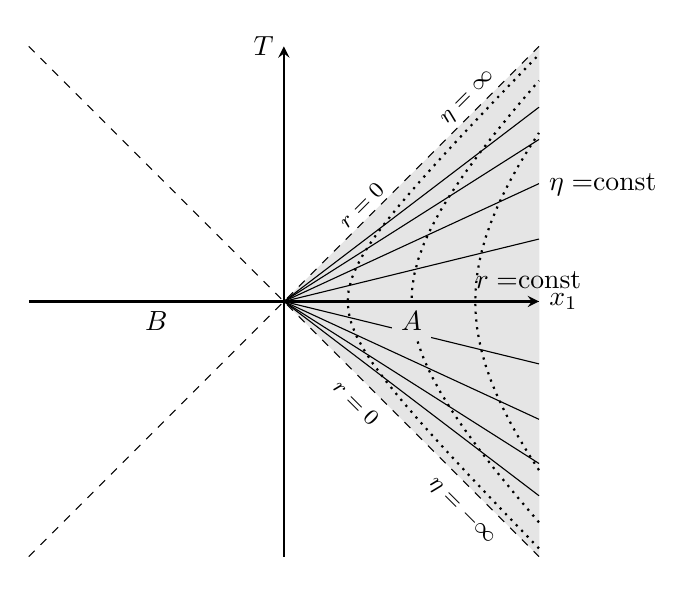
\begin{tikzpicture}[%
    scale=2.7,%
    maingrid/.style={draw,very thick},%
    subgrid/.style={draw,thin},%
    tlabels/.style={pos=0.88,above,sloped,yshift=-.3ex},%
    label/.style={%
        postaction={%
            decorate,%
            transform shape,%
            decoration={%
                markings,%
                mark=at position .65 with \node #1;%
            }%
        }%
    },%
]%
    \pgfmathdeclarefunction{arcosh}{1}{\pgfmathparse{ln(#1+sqrt(#1+1)*sqrt(#1-1))}}
    \pgfmathsetmacro{\Xmax}{1.2}
    \pgfmathsetmacro{\Tmax}{1.2}
    \pgfmathsetmacro{\g}{1}
    \newcommand\mylabelstyle\footnotesize
    
    \fill[black!10] (-45:1.7)--(0,0)--(45:1.7)--cycle;
    
    % curves t=constant
    \foreach \t in {-1,-0.75,...,1}{%
        \path[subgrid] (0,0) -- (\Xmax,{\Xmax*tanh(\g*\t)});
    }

    % curves x=constant
    \foreach \xx in {0.3,0.6,...,\Xmax}{%
        \path[draw,thick,dotted]
            plot[domain=-{arcosh(\Xmax/\xx)/\g}:{arcosh(\Xmax/\xx)/\g}]
            ({\xx*cosh(\g*\x)},{\xx*sinh(\g*\x)});  
    }

    % X-axis, T-axis, and dashed lines t=+/-infty 
    
    \draw[thick,-stealth] (-\Xmax,0) -- (\Xmax,0) node[right] {$x_1$}
    	node[pos=0.75,below,fill=black!10] {$A$}
	node[pos=0.25,below,fill=white] {$B$};
    \draw[thick,-stealth] (0,-\Tmax) -- (0,\Tmax) node[left] {$T$};
    \draw[dashed] (-\Xmax,-\Tmax) -- (\Xmax,\Tmax) 
        node[pos=0.67,above,sloped,yshift=-.3ex] {\mylabelstyle$r=0$}
        node[tlabels,black] {\mylabelstyle$\eta=\infty$};
    \draw[dashed] (-\Xmax,\Tmax) -- (\Xmax,-\Tmax) 	
    	node[pos=0.67,below,sloped,yshift=-.3ex] {\mylabelstyle$r=0$}
        node[tlabels,black,below] {\mylabelstyle$\eta=-\infty$};
    \node at (1.5, 0.55) {$\eta=$const};
    \node at (1.15, 0.1) {$r=$const};
\end{tikzpicture}
\caption{\label{fig:Rindler} The Rindler spacetime (shaded region) embedded in the Minkowski spacetime.}
\end{figure}


Now we want to give a concrete expression of the modular Hamiltonian $H_A$ defined by Eq.\,\eqref{Gibbs_State} for the Rindler observer.
In order to fix its form, we consider the matrix element of the reduced density matrix $\rho_A$,
\begin{align}
	\langle \phi_A' | \rho_A | \phi_A \rangle = \frac{1}{Z}\, \langle \phi_A' | e^{-2\pi\, H_A} | \phi_A \rangle  \ ,
\end{align}
and regard the right-hand side as a transition amplitude from an initial state $|\phi_A\rangle$ to a final state $|\phi_A'\rangle$.
The (Euclidean) ``time" evolution is generated by the modular Hamiltonian $H_A$ over the period $2\pi$.
Looking back to the example in the previous subsection, we can understand that the system on the region $A$ is time evolved along the angular direction $\tau$ starting from $\tau=0$ to $2\pi$ (see Fig.\,\ref{fig:ScalarInfinite}).
We thus conclude the modular Hamiltonian in the present case is the generator of the translation along the modular time $\tau$, hence $H_A = \partial_\tau$.\footnote{In Lorentzian signature, the modular Hamiltonian generates the boost $K = \partial_\eta$ in the Rindler spacetime.}
In Euclidean QFT, the modular Hamiltonian is written explicitly by the Noether's theorem as
\begin{align}\label{Modular_Hamiltonian}
	H_A = \int_{x_0=0, x_1\ge 0} \d^{d-1}x\, x_1\, T_{00} \ ,
\end{align}
where $T_{\mu\nu}$ is the stress tensor, which will be defined in Eq.\,\eqref{STDef}.
This result is a particular case of the theorem by \textcite{Bisognano:1976za,Bisognano:1975ih} that is valid for any QFT even with interactions.


Recalling the construction of the thermofield double state Eq.\,\eqref{TFD}, we can rewrite the ground state wave function in the Minkowski spacetime in the following form,
\begin{align}
		\Psi [\phi_A, \phi_B] = \frac{1}{\sqrt{Z}} \sum_{n}\,e^{-\beta E_n/2} \varphi_n [\phi_A]\, \varphi_n [\phi_B] \ ,
	\end{align}
where $\phi_A$ and $\phi_B$ are states on the time slice $A$ and $B$ respectively, and $\varphi_n [\phi]$ is the $n^{th}$ eigenfunction of the modular Hamiltonian $H_A$ with eigenvalue $E_n$.
Namely, we are able to \emph{purify} a mixed state in the Rindler spacetime  to a pure state in the Minkowski spacetime by viewing the region inside the Rindler horizon as a fictitious system \cite{Israel:1976ur,Laflamme:1988wg}.




\subsection{Structure of UV divergences}\label{ss:UVstructure}
In the previous section, we rewrite the definition of entanglement entropy in terms of an Euclidean effective action $\log Z_n$ on an $n$-fold cover $\CM_n$ with a conical singularity along a codimension-two surface $\Sigma = \partial A$ surrounding the region $A$ of interest.
In QFT on a curved spacetime, the effective action is regarded as a function of the metric $g_{\mu\nu}$ on $\CM_n$; thus we are able to classify the UV divergent terms by diffeomorphism invariant local terms.
Here we restrict our attention to QFTs without dimensionful parameters (= CFTs) for simplicity, whose effective action may be given by\footnote{One can repeat the same argument presented here for any renormalizable QFTs with a slight modification. For example, one can add terms $\Lambda^{d-2}\,M^2, \Lambda^{d-4}\, M^2\, \CR, \cdots$ to the integrand if $M$ is a parameter of mass dimension one.
This does not change the UV structure, and we ignore them for the moment.
}
\begin{align}\label{PF_UV}
\begin{aligned}
\log Z_n [g_{\mu\nu}] =&\, \sum_{i=0}^{\left[ d/2\right]} C_{d-2i} \int_{\CM_n} \d^d x\, \sqrt{g}\, \Lambda^{d-2i}\, \CR^i \\
	& + (-1)^{\frac{d-1}{2}}F[g_{\mu\nu}] \ ,
\end{aligned}
\end{align}
where $\Lambda$ is the UV cutoff scale of mass dimension one and $\CR^i$ is a scalar polynomial of the Riemann tensors of order $i$ on $\CM_n$.
We call $F[g_{\mu\nu}]$ the renormalized free energy that is dimensionless and a scheme-independent nonlocal functional of the metric in odd dimensions.
In contrast, there is a logarithmic divergence $\sim C_0 \log \Lambda$ in addition to Eq.\,\eqref{PF_UV} in even dimensions, which makes the renormalized free energy ambiguous.
It is actually the source of the conformal anomaly and the coefficient $C_0$ depends on the central charges when the theory is conformally invariant.


We put aside the logarithmic divergence for a moment and determine the general structure of the UV divergences of entanglement entropy.
We plug the general form Eq.\,\eqref{PF_UV} into Eq.\,\eqref{EE_PF}, where there appears only the difference $\log Z_n - n\log Z$ of the effective actions for $n$ close to $1$.
The UV divergent term of order $\Lambda^{d-2i}$ is proportional to the integral\footnote{We often use the shorthand notation for an integral $\int_{\CM} \equiv \int_{\CM} \d^d x\,\sqrt{g}$ with the measure suppressed.} $\int_{\CM_n}\CR^i - n \int_{\CM}\CR^i$ that should localize on the entangling surface $\Sigma$ since the $n$-fold covering space $\CM_n$ differs from the original space $\CM$ only around $\Sigma$.
Especially, the leading divergence with $i=0$ cancels out because of $\text{Vol}(\CM_n) = n\, \text{Vol} (\CM_1)$.
We thus end up with the UV divergences in the entanglement entropy starting from $O(\Lambda^{d-2})$:
\begin{align}\label{UV_structure}
S_A = c_{d-2}\,\Lambda^{d-2} + c_{d-4}\, \Lambda^{d-4} + \cdots \ ,
\end{align}
where $c_{d-2i}$ are given by the integrals of local diffeomorphism invariants on $\Sigma$, schematically written as
\begin{align}\label{UV_coeff}
	c_{d-2i} = \sum_{l+m=i-1}\int_\Sigma \, \CR^l\, \CK^{2m} \ ,
\end{align}
where $\CK$ is the extrinsic curvature of $\Sigma$ of the order of $2m$, whose definition will be given in Eq.\,\eqref{ExtrinsicCurvature},
and $\CR^l\, \CK^{2m}$ are scalar polynomials of $\CR$ and $\CK$ of the order of $l$ and $2m$ respectively.
The reason only even powers of the extrinsic curvatures appear in Eq.\,\eqref{UV_coeff} is that the entanglement entropy for a region $A$ is equal to that of its complement $\bar A$ while their extrinsic curvatures have opposite signs, hence the odd powers of $\CK$ vanish.

We derived the UV structure Eq.\,\eqref{UV_structure} assuming the covariance and renormalizability of QFTs on a manifold without boundaries.
If we relax the assumptions, there are a variety of cases where entanglement entropy can take a different UV structure.
For instance, nonrelativistic systems with Fermi surfaces have the entanglement entropy that violates the area law logarithmically \cite{Wolf:2006zzb,Gioev:2006zz} [see also \textcite{Ogawa:2011bz,Huijse:2011ef} for the holographic descriptions].
For nonsmooth entangling surfaces such as those with corners and wedges, the entanglement entropies have additional UV divergences whose coefficients depend on the opening angles \cite{Fradkin:2006mb,Casini:2006hu,Hirata:2006jx,Casini:2008as,Bueno:2015xda,Bueno:2015rda,Elvang:2015jpa,Klebanov:2012yf,Myers:2012vs}.\footnote{See also \textcite{Ghasemi:2017pke} for a more recent work.}


The general structure Eq.\,\eqref{UV_structure} guarantees the UV finiteness of the mutual information $I(A,B)$ of two disjoint systems $A$ and $B$ defined by Eq.\,\eqref{MI} because every coefficient $c_{d-2i}$ of the UV divergent term $\Lambda^{d-2i}$ of the entanglement entropy is given by an integral on the entangling surface and they cancel in the mutual information due to the trivial identity (see Fig.\,\ref{fig:MI})
\begin{align}
	\int_{\Sigma_{A+B}} = \int_{\Sigma_A} + \int_{\Sigma_B} \ .
\end{align}


We fix the precise forms of the coefficients for free fields in the next Sec. \ref{ss:HeatKernel}.
Note that there is a logarithmic divergence in even dimensions which we separately deal with when we discuss CFT in Sec. \ref{ss:CFT}.

\endinput